\documentclass[preview,float]{standalone}
\usepackage{tikz}
\usetikzlibrary{hobby,decorations.markings}
\usepackage{graphicx}
\usepackage{nicefrac}
\usepackage{amsmath}

\begin{document}
\begin{tikzpicture}
%AXIS
    \draw [<->,thick] (-0.3,0.1) node (yaxis) [above] {$y$}
    |- (0.2,-0.5) node (xaxis) [right] {$x$};
% CAR
\draw[green,
  postaction={
    decorate,
    decoration={
      markings,
      mark=between positions 0 and 1 step 0.33 with
      {
        \node[transform shape] {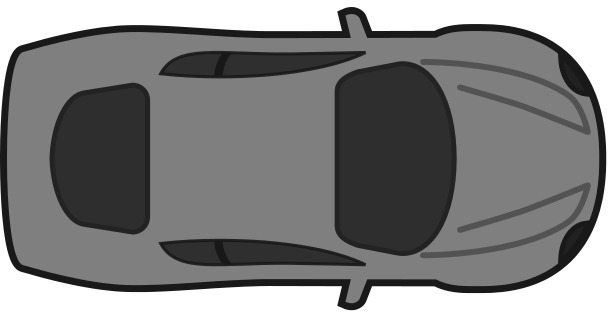
\includegraphics[width=.5cm]{car}};
      }
    }
  }
]
(0.75,0);
%CONSTRAINTS CAR X AXIS
\draw [<->,semithick,>=stealth] (1,-0.2) to (2.55,-0.2);
\draw(1.2,-0.4) node {$x_{\min}$};
\draw(2.65,-0.4) node {$x_{\max}$};

%CONSTRAINTS OBSTACLE Y AXIS
\draw [<->,semithick,>=stealth] (3.6,0.0) to (3.6,0.6);
\draw [<->,semithick,>=stealth] (3.6,0.0) to (3.6,-0.6);
\draw(4,-0.4) node {$\nicefrac{-W}{2}$};
\draw(4,0.38) node {$\nicefrac{W}{2}$};

%CONSTRAINTS OBSTACLE DASHED
\draw [-,dashed,very thick] (1,0) to (2.55,0.2);

%REGION
\draw [-,semithick,green] (1,0.015) to (2.55,0.215);
\draw [-,semithick,green] (2.55,0.215) to (2.55,0.59);
\draw [-,semithick,green] (2.55,0.59) to (1,0.59);
\draw [-,semithick,green] (1,0.59) to (1,0.01);
%SAFE SPACE OBSTACLE
\draw [red, thick, dashed] (2.55,0.2) rectangle (3.45,-0.2);

%OBSTACLE
\draw[red,
postaction={
	decorate,
	decoration={
		markings,
		mark=between positions 0 and 1 step 0.5 with
		{
			\node[transform shape] {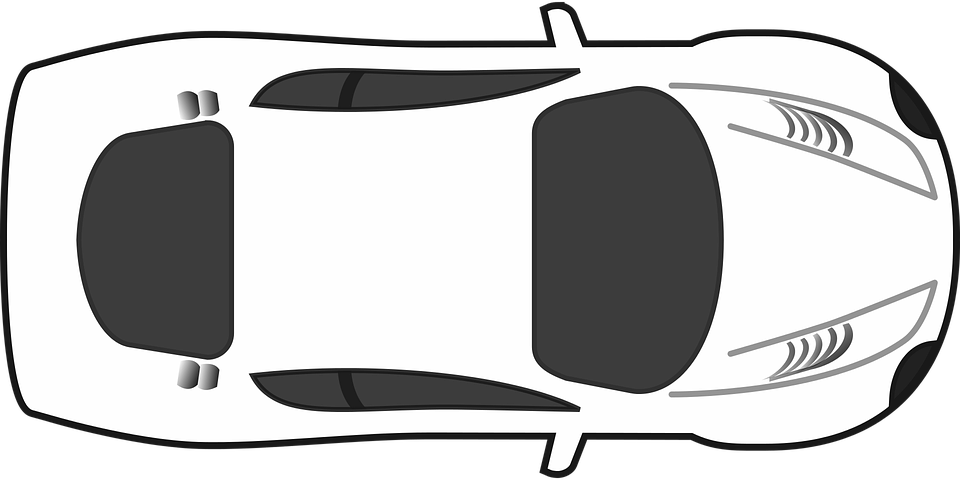
\includegraphics[width=.5cm]{obstacle}};
		}
	}
}
]
(3,0);


%ROAD
\draw[dashed,ultra thin]
(-0.5,0.2) to[out angle=0,in angle=180] (4.5,0.2);
\draw[dashed,ultra thin]
(-0.5,-0.2) to[out angle=0,in angle=180] (4.5,-0.2);
\draw
(-0.5,0.6) to[out angle=0,in angle=180] (4.5,0.6);
\draw
(-0.5,-0.6)to[out angle=0,in angle=180] (4.5,-0.6);
\end{tikzpicture}
\end{document}